\chapter{Design and Implementation}

(approx. 10 pages)\\

* Check if you have addressed Provided a graphical representation for your design?\\
* Provided a Project folders and files diagram?\\

\section{Program Design and Interaction Mechanisms} %TODO: Everybody, yeaahhhh ;)
* Approach to design\\
* important issues and choices and their relationships to theoretical concepts and the hardware and software platforms\\
* Did you use the GPIO module? How? In terms of interrupts and the setup in the main\\
* Did you use interrupts? How?\\ 
* Did you use multiple threads / handlers? How? Why?\\
* Did you use TI-RTOS? How?\\

\section{Main Functions and State Machine} %TODO: Hendrik

\begin{figure}[H]
	\begin{center}
		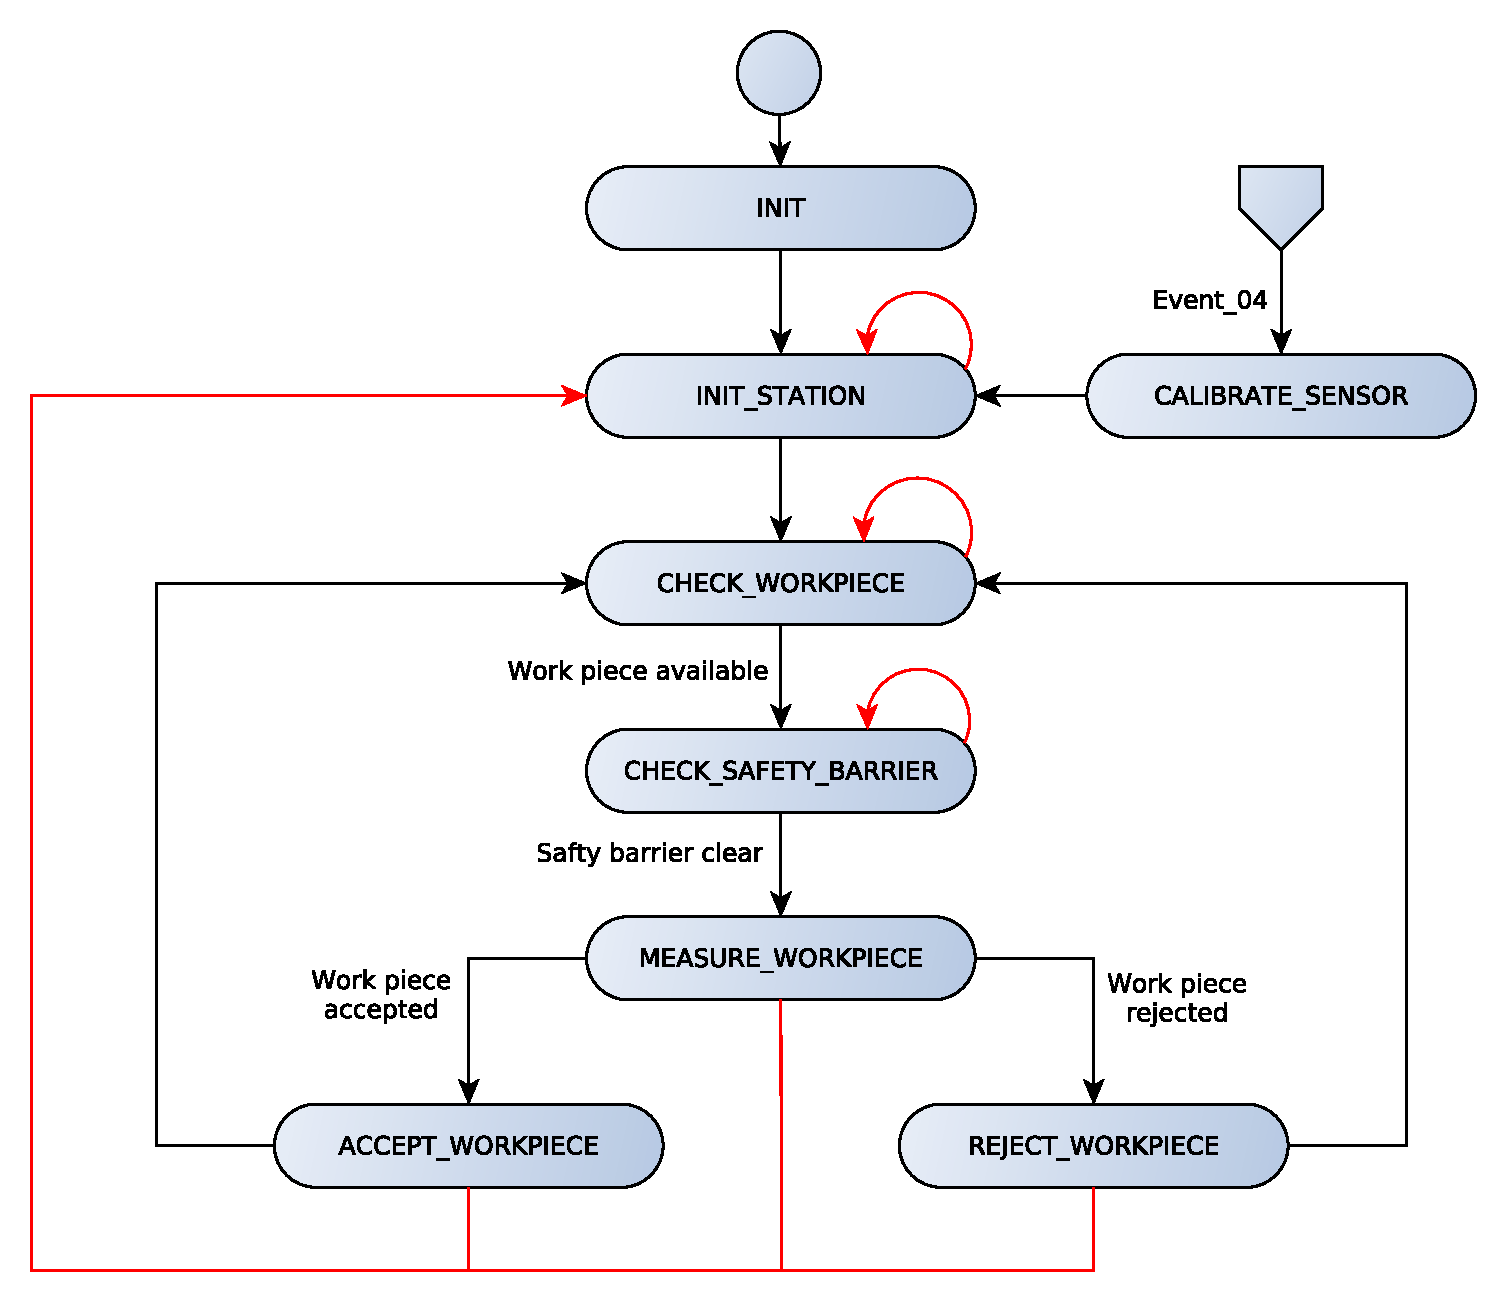
\includegraphics[scale=.60]{media/StateMachine_Main.pdf} 	
		\caption{Main State Machine}
		\label{fig:statemachine}
	\end{center}
\end{figure}

\section{Device Driver Library} %TODO: Timo
* Did you use the GPIO module? How? Through the qut library... Pin Map table?\\
* Did you use the ADC? How? 

% TODO: Table of measurements?

\begin{figure}[H]
	\begin{center}
		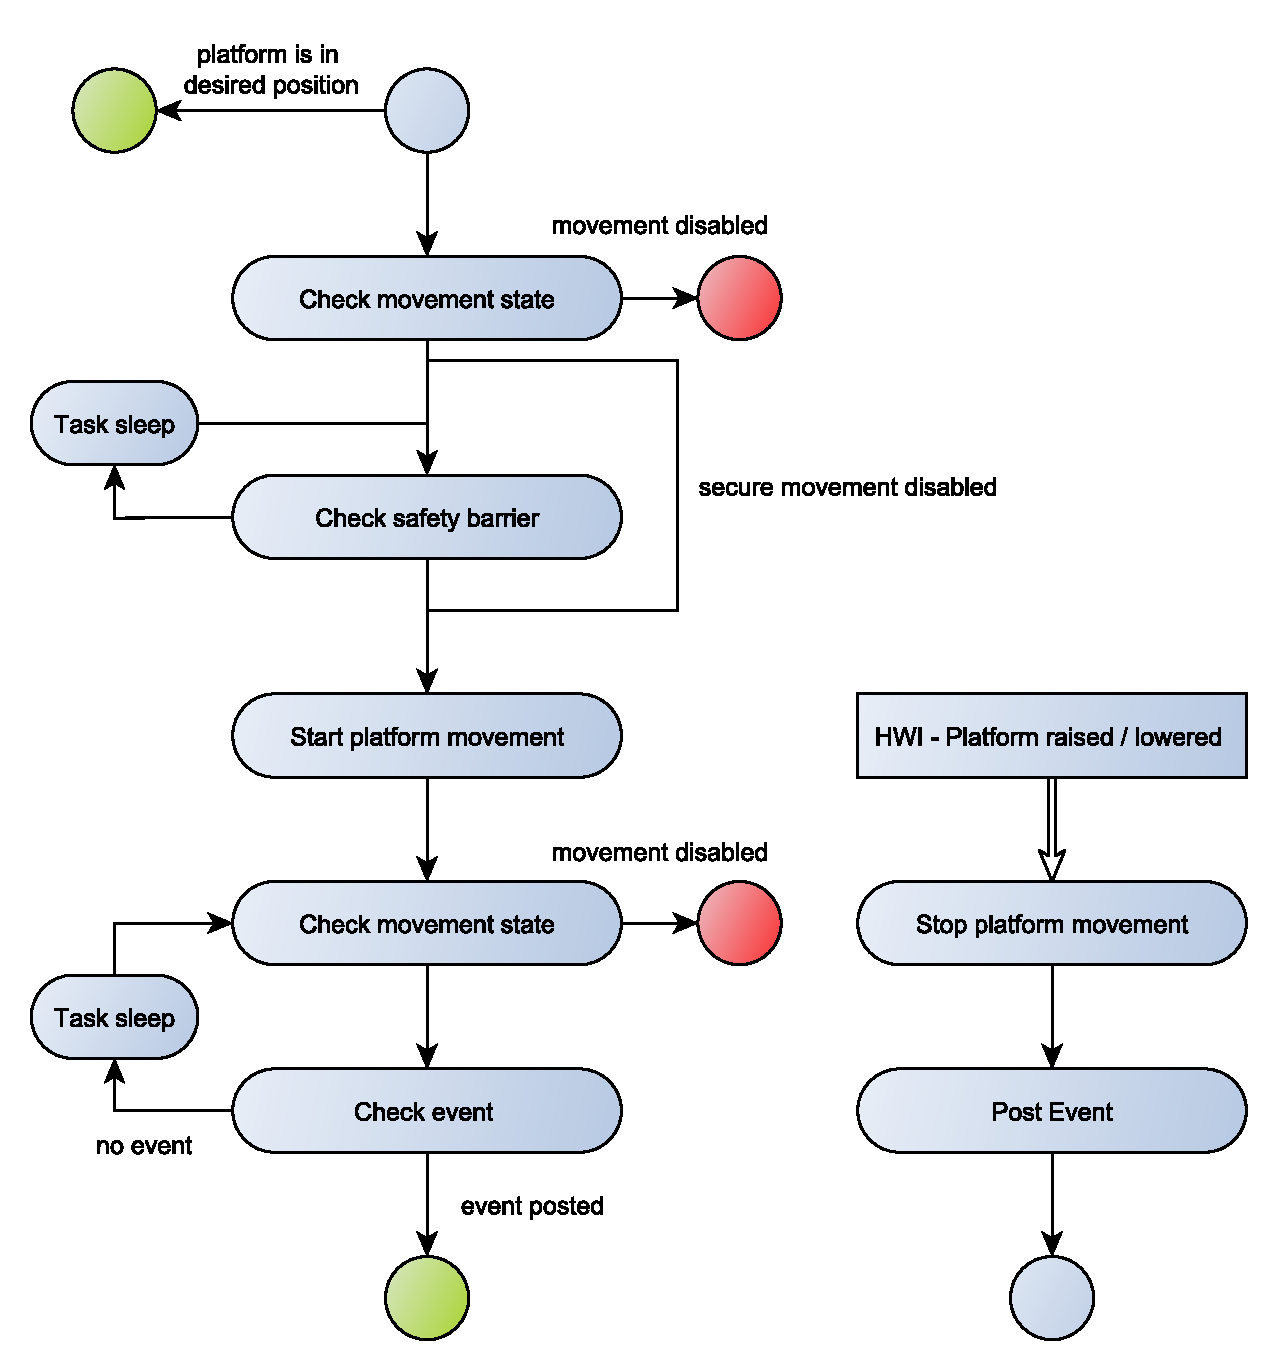
\includegraphics[scale=.60]{media/Flow_Chart_MovePlatform.pdf} 	
		\caption{Flow Chart Move Platform}
		\label{fig:moveplatform}
	\end{center}
\end{figure}

\section{User Interface} %TODO: Pixel-Julian

In order to transfer data from the state machine to the display logic, a C struct called \texttt{festoData} is introduced. All the data that is needed to display is represented in that struct. Its internal representation is shown in listing \ref{struct}. Apart from the values of the current and the operating time, it includes the actual state of the screen as well as the measurements that are received during the automated processing of workpieces.

\begin{lstlisting}[label=struct, caption=festoData struct, style=customc]
typedef struct
{
	time_t 			theTime;
	uint32_t 		operatingTime;
	
	screenState_type 	screenState;
	thresholdState_type	thresholdState;
	calibrateState_type	calibrateState;
	
	material_type 		currentMaterial;
	color_type 		currentColor;
	uint32_t 		currentHeight;
	
	uint32_t		countTotal;
	uint32_t 		countAccepted;
	uint32_t 		countMetallic;
	uint32_t 		countBlack;
	
	uint32_t 		thresholdTop;
	uint32_t 		thresholdBottom;
	
	uint32_t 		calibrateFirst;
	uint32_t 		calibrateSecond;
	
	bool 			enableMovement;
	bool 			measuring;
} festoData_type;
\end{lstlisting}

These values are accessed and written by either the state machine or the button handler. No value is modified by both. 


The \texttt{updateScreenTask} is responsible for painting a new frame with updated values onto the screen.
It waits until the \texttt{Event\_Id\_06} is posted and then calls the corresponding drawing function.

This event itself is posted whenever the eventHandler adjusts the data that is part of the \texttt{festoData} struct.
This could for example be an adjustment of the current time or of the state of the screen.

There are three different screen states while each one of them is allowing the user to perform different actions. They are shown in figure \ref{fig:gui}.

\begin{figure} [H] 	
	\begin{center}
		\subfigure[Status]{\includegraphics[width=0.30\textwidth]{media/Screenshot0.png}
			\label{fig:guiStatus}} 
		\quad
		\subfigure[Calibration]{\includegraphics[width=0.30\textwidth]{media/Screenshot1.png}
			\label{fig:guiCalibrate}} 
		\quad
		\subfigure[Threshold]{\includegraphics[width=0.30\textwidth]{media/Screenshot2.png}
			\label{fig:guiThreshold}} 
		\caption{GUI Screenshots}
		\label{fig:gui}
	\end{center}
\end{figure} 

The first display state shown in figure \ref{fig:guiStatus} is the status screen.
It shows all the values of the last measured workpiece and furthermore a summary of all the measured workpieces in total.
In addition, the total runtime and the current flow-rate are displayed.
While this screen is active, the two buttons on the left allow for switching into another screen state, while the button on the right starts and stops the automation process of the measuring.

When the user goes into the calibration mode, the current values and the summary disappear and he is then asked to enter the height for the workpieces that will be used for calibration, as shown in figure \ref{fig:guiCalibrate}.
In this screen the buttons on the left are either used to switch again into another screen state or to adjust the calibration values.
The button on the right consecutively continues the calibration process.

Finally, the last screen state is the threshold mode.
As in the calibration mode, two values are displayed which can as well be adjusted by the user while using the buttons on the left.
The button on the right is again used for continuing and confirming.
All the workpieces that are measured in the automation process are compared against these values and will only be accepted if their height value is between these thresholds.

The drawing of the screen itself is done via the \texttt{updateScreen} function in the \texttt{screen.c} file.
At first the screen is cleared by painting a rectangle with the color of the background over the whole screen.
Afterwards a distinction of cases decides which screen is to be drawn.
With help of the functions \texttt{GrStringDraw} and \texttt{GrStringDrawCentered}  by the \textit{TivaWare™ Graphics Library} the strings will then be printed at the appropriate coordinates. 
Additionally the rectangles are drawn with the help of the \texttt{GrRectDraw} function.
